\documentclass[times, utf8, diplomskirad]{fer}
% Dodaj opciju upload za generiranje konačne verzije koja se učitava na FERWeb
% Add the option upload to generate the final version which is uploaded to FERWeb

\usepackage{booktabs}
\usepackage{float}
\usepackage[bottom]{footmisc}
\usepackage{algpseudocode}
\usepackage{amsfonts}
\usepackage{pythonhighlight}
\usepackage{blindtext}


%--- PODACI O RADU / THESIS INFORMATION ----------------------------------------

% Naslov na engleskom jeziku / Title in English
\title{Visual state representation of robot manipulator}

% Naslov na hrvatskom jeziku / Title in Croatian
\naslov{Vizualna reprezentacija stanja robotskog manipulatora}

% Broj rada / Thesis number
\brojrada{476}

% Autor / Author
\author{Sven Šćekić}

% Mentor 
\mentor{Prof.\@ Marija Seder}

% Datum rada na engleskom jeziku / Date in English
\date{June, 2024}

% Datum rada na hrvatskom jeziku / Date in Croatian
\datum{lipanj, 2024.}

%-------------------------------------------------------------------------------


\begin{document}


% Naslovnica se automatski generira / Titlepage is automatically generated
\maketitle


%--- ZADATAK / THESIS ASSIGNMENT -----------------------------------------------

% Zadatak se ubacuje iz vanjske datoteke / Thesis assignment is included from external file
% Upiši ime PDF datoteke preuzete s FERWeb-a / Enter the filename of the PDF downloaded from FERWeb
\zadatak{diplomski-zadatak.pdf}


%--- ZAHVALE / ACKNOWLEDGMENT --------------------------------------------------

\begin{zahvale}
  % Ovdje upišite zahvale / Write in the acknowledgment
    OVDJE IDU ZAHVALE
\end{zahvale}


% Odovud započinje numeriranje stranica / Page numbering starts from here
\mainmatter


% Sadržaj se automatski generira / Table of contents is automatically generated
\tableofcontents


%--- UVOD / INTRODUCTION -------------------------------------------------------
\chapter{Uvod}
\label{pog:uvod}
\hspace{\parindent}Robotika i automatika u današnjem svijetu dobivaju sve više pozornosti zbog svojih brojnih mogućnosti koje pružaju.
Neke od najvećih industrija čiji je rast značajno potpomognut razvojem robotike su automobilska i zdravstvena industrija.
Zbog primjene u takvim industrijama zahtjeva se poznavanje točne konfiguracije robota sa svim potrebnim parametrima kako
bi se zadane radnje koje bi roboti trebali izvoditi izvele točno onako kako je očekivano.
Ovo je posebice bitno u zdravstvenoj industriji gdje male razlike u parametrima mogu rezultirati ozbiljnim posljedicama.

U ovom diplomskom radu pobliže ćemo objasniti što sve čini konfiguraciju robota te kako se ona zapisuje u standardnom obliku.
Objasnit ćemo što su direktna i inverzna kinematika te kako se koriste prilikom prikaza različitih stanja robota.
Nadalje ćemo prikazati različite metode za generiranje 2D slika pomoću 3D modela robota i njegovih konfiguracija.
Na kraju ćemo prikazati suprotan proces, odnosno kako možemo iskoristit duboke modele kako bi iz njih naučili 3D model robota.
Tijekom cijelog rada ove metode primjenjivat ćemo na Franka Emika Panda robotskom manipulatoru, ali naravno one su primjenjive i na bilo kojem drugom.

%-------------------------------------------------------------------------------
\chapter{Kinematika robota}
Kinematika je, uz statiku i dinamiku, jedna od tri osnovne grane mehanike.
Kinematika opisuje kretanje tijela ne uzimajući u obzir sile koje uzrokuju kretanje.
Statika proučava tijela u ravnoteži, odnosno sile koje održavaju tijelo ravnotežnom položaju, dok dinamika proučava kretanje objekata prilikom djelovanja različitih sila.

Kada pri kretanju tijela iz analize uklonimo sve popratne sile tada je njegovo gibanje određeno funkcijom kutova između njegovih dijelova.
Kroz ovaj rad ćemo promatrati kinematiku u kontekstu robotskog manipulatora te kako je njegovo gibanje određeno ponašanjem njegovih zglobova i članaka.

\section{Robotski manipulator}
Robotski manipulator je specijalizirana vrsta robota dizajniran za obavljanje određenih zadataka.
Koristi se u različitim industrijama zbog svojih mogućnosti da precizno obavlja zadane radnje.
Sastoji se od zglobova (eng. \textit{joints}) koji svojom rotacijom ili pomicanjem u prostoru omogućuju da manipulator postigne zadano stanje.
Zglobovi su međusobno povezani člancima (eng. \textit{links}) koji imaju svoju određenu duljinu.

Na samom vrhu robotskog manipulatora nalazi se izvršni element (eng. \textit{end effector}) koji služi za interakciju sa stvarnim svijetom.
Upravo je taj dio zadužen za obavljanje zadanih radnji.
Na slici \ref{fig:panda-zglob} možemo vidjeti pirmjere zglobova i članaka na Panda robotskom manipulatoru kojeg ćemo promatrati tijekom ovog rada.
\begin{figure}[H]
    \centering
    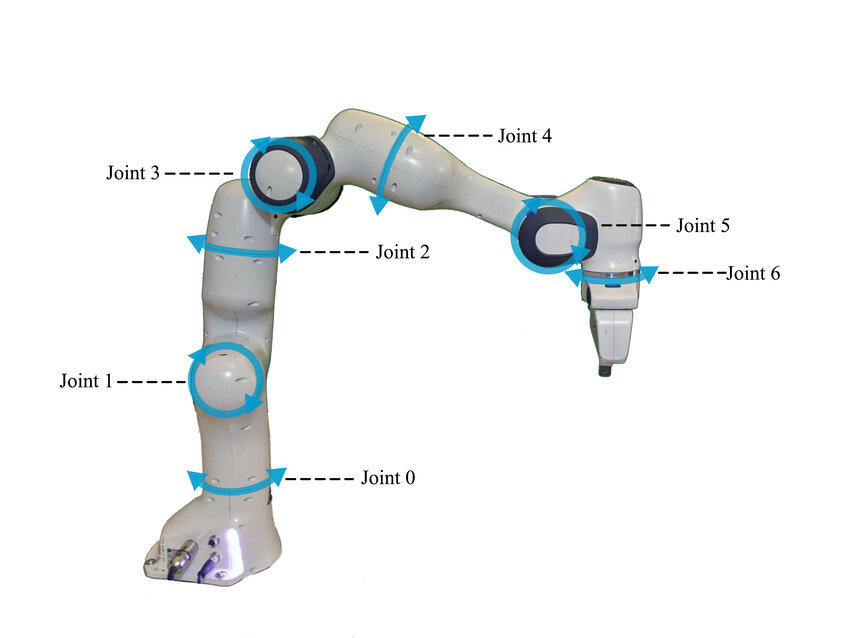
\includegraphics[width=12cm]{img/panda-links-and-joints}
    \caption{Zglobovi i članci na Frank Emika Panda manipulatoru\protect\footnotemark}
    \label{fig:panda-zglob}
\end{figure}
\footnotetext{Preuzeto sa \url{ https://www.researchgate.net/ }}

\subsection{Konfiguracija manipulatora}
Konfiguraciju manipulatora čini potpuno određen položaj svih njegovih točaka.
Skup svih mogućih konfiguracija čini konfiguracijski prostor manipulatora.
Pojedinu konfiguraciju tada možemo promatrati kao točku unutar konfiguracijskog prostora.

Kao i svaki prostor i konfiguracijski prostor ima svoju dimenziju i oblik.
Dimenzija je određena brojem realnih koordinata potrebnih za potpunu reprezentaciju konfiguracije, što još nazivamo i stupnjevi slobode.
Oblik konfiguracijskog prostora je također jako bitan s obzirom da on određuje moguće prepreke i ograničenja unutar samog prostora što smanjuje broj mogućih konfiguracija
U nastavku ćemo pobliže objasniti što sve utječe na broj stupnjeva slobode manipulatora te kakve sve oblike konfiguracijskog prostora možemo susresti.

\subsection{Vrste zglobova i stupnjevi slobode}
Zglobovi i članci zajedno omogućuju da manipulator postigne željena stanja.
Skup svih stanja koje manipulator može dosegnuti u prostoru nazivamo radni prostor robota (eng. \textit{workspace}).
Ono što najviše određuje radni prostor jesu vrste zglobova od kojih se naš manipulator sastoji.

\begin{figure}[H]
    \centering
    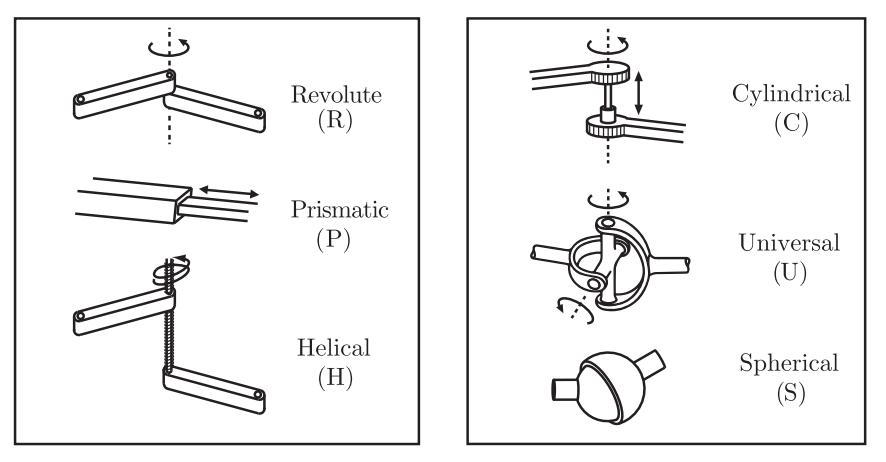
\includegraphics[width=12cm]{img/robot-joints}
    \caption{Vrste zglobova}
    \label{fig:robot-joints}
\end{figure}
\footnotetext{Preuzeto sa \url{ https://hades.mech.northwestern.edu/images/2/25/MR-v2.pdf }}
Na slici \ref{fig:robot-joints} možemo vidjeti različite vrste zglobova koje se koriste.
Svaki od ovih zglobova sastoji se od određenog broja stupnjeva slobode.
Stupnjeve slobode čini broj nezavisnih varijabli koje određuju kretanje nekog tijela.
Kruta tijela u prostoru obično sadrže šest stupnjeva slobode.
Tri stupnja slobode za translaciju, odnosno rotaciju, po svakoj od triju koordinatnih osi.

Kod robotskih manipulatora stupnjeve slbode definiramo na razini zglobova ili manipulatora u cijelosti.
Tako revolucijski zglob sadrži jedan stupanj slobode, odnosno rotaciju oko jedne osi, dok sferični zglob sadrži 3 stupnja slobode te funkcijom podjseća na ljudski rameni zglob.
Ako želimo izraziti broj stupnjeva slobode za manipulator u cijelosti tada se možemo poslužiti Grüblerovom formulom koju možemo vidjeti u formuli (\ref{eq:grubler}).
Varijabla \textit{m} predstavlja konstantu, koja iznosi 3 za planarne manipulatore, odnosno 6 za prostorne manipulatore.
Varijabla \textit{N} predstavlja broj članaka, dok varijabla \textit{J} predstavlja broj zglobova.
Konačno, varijabla \textit{f\textsubscript{i}} predstavlja broj stupnjeva slobode pojedinog zgloba.

\begin{equation}
    \begin{aligned}
        \text { dof } &=\underbrace{m(N-1)}_{\text {rigid body freedoms }}-\underbrace{\sum_{i=1}^{J} c_{i}}_{\text {joint constraints }} \\
        &=m(N-1)-\sum_{i=1}^{J}\left(m-f_{i}\right) \\
        &=m(N-1-J)+\sum_{i=1}^{J} f_{i} \cdot
    \end{aligned}
    \label{eq:grubler}
\end{equation}

\subsection{Vrste konfiguracijskog prostora}

%-------------------------------------------------------------------------------
\chapter{Rezultati i rasprava}
\label{pog:rezultati_i_rasprava}



%--- ZAKLJUČAK / CONCLUSION ----------------------------------------------------
\chapter{Zaključak}
\label{pog:zakljucak}



%--- LITERATURA / REFERENCES ---------------------------------------------------

% Literatura se automatski generira iz zadane .bib datoteke / References are automatically generated from the supplied .bib file
% Upiši ime BibTeX datoteke bez .bib nastavka / Enter the name of the BibTeX file without .bib extension
\bibliography{literatura}



%--- SAŽETAK / ABSTRACT --------------------------------------------------------

% Sažetak na hrvatskom
\begin{sazetak}
  Unesite sažetak na hrvatskom.

  \blindtext
\end{sazetak}

\begin{kljucnerijeci}
  prva ključna riječ; druga ključna riječ; treća ključna riječ
\end{kljucnerijeci}


% Abstract in English
\begin{abstract}
  Enter the abstract in English.
  
  \blindtext 
\end{abstract}

\begin{keywords}
  the first keyword; the second keyword; the third keyword
\end{keywords}


%--- PRIVITCI / APPENDIX -------------------------------------------------------

% Sva poglavlja koja slijede će biti označena slovom i riječi privitak / All following chapters will be denoted with an appendix and a letter
\backmatter

\chapter{The Code}

\Blindtext


\end{document}
